\documentclass[12pt,a4paper]{article}
\usepackage[latin1]{inputenc}
\usepackage[spanish]{babel}
\usepackage{amsmath}
\usepackage{amsfonts}
\usepackage{amssymb}
\usepackage{graphicx}
\usepackage[usenames]{color}
\usepackage{xcolor}
\usepackage[spanish, onelanguage, linesnumbered,lined,boxed,commentsnumbered]{algorithm2e}

% Default fixed font does not support bold face
\DeclareFixedFont{\ttb}{T1}{txtt}{bx}{n}{12} % for bold
\DeclareFixedFont{\ttm}{T1}{txtt}{m}{n}{12}  % for normal
% Custom colors
\usepackage{color}
\definecolor{deepblue}{rgb}{0,0,0.5}
\definecolor{deepred}{rgb}{0.6,0,0}
\definecolor{deepgreen}{rgb}{0,0.5,0}

\usepackage{listings}

% Python style for highlighting
\newcommand\pythonstyle{\lstset{
language=Python,
basicstyle=\ttm,
otherkeywords={self},             % Add keywords here
keywordstyle=\ttb\color{deepblue},
emph={MyClass,__init__},          % Custom highlighting
emphstyle=\ttb\color{deepred},    % Custom highlighting style
stringstyle=\color{deepgreen},
frame=tb,                         % Any extra options here
showstringspaces=false            % 
}}


% Python environment
\lstnewenvironment{python}[1][]
{
\pythonstyle
\lstset{#1}
}
{}

% Python for external files
\newcommand\pythonexternal[2][]{{
\pythonstyle
\lstinputlisting[#1]{#2}}}

% Python for inline
\newcommand\pythoninline[1]{{\pythonstyle\lstinline!#1!}}




\newcommand{\forcond}{$i=0$ \KwTo $n$}
\SetKwFunction{FRecurs}{FnRecursive}%
\SetKwFunction{selectionSort}{selectionSort}

\SetKwFunction{insertionSort}{insertionSort}
\SetKwFunction{quickSort}{quickSort}
\SetKwFunction{bubbleSort}{bubbleSort}
\SetStartEndCondition{ }{}{}%
\SetKwProg{Fn}{def}{\string:}{}
\SetKwFunction{Range}{range}%%
\SetKw{KwTo}{en}\SetKwFor{For}{Para}{\string:}{}%
\SetKwIF{If}{ElseIf}{Else}{Si}{:}{Sino, Si}{en caso contrario:}{}%
\SetKwFor{While}{Mientras}{:}{fin}%
\renewcommand{\forcond}{$i$ \KwTo\Range{$n$}}
\AlgoDontDisplayBlockMarkers\SetAlgoNoEnd\SetAlgoNoLine
\AlgoDisplayBlockMarkers\SetAlgoBlockMarkers{ }{ }%
\SetAlgoNoEnd
\SetKw{Return}{Regresar}%

\usepackage[left=2cm,right=2cm,top=2cm,bottom=2cm]{geometry}
\author{
Jos\'e Manuel Tapia Avitia.\\
Matr\'icula: 1729372\\ 
\texttt{jose.tapiaav@gmail.com}\\
\texttt{https://github.com/jose-tapia/1729372MC}
}
\title{Reporte de algoritmos de ordenamiento}

\begin{document}
\maketitle

El presente reporte tiene la finalidad de mostrar a grandes rasgos las caracteristicas principales y el funcionamiento de algunos algoritmos de ordenamiento.

\section{$\textcolor{blue}{\mathrm{SelectionSort}}$}
El algoritmo de selecci\'on es el que a mi consideraci\'on es el m\'as intuitivo.
\newline
Al inicio, busca el menor elemento (de acuerdo a nuestra funci\'on de comparaci\'on) y lo intercambia por el elemento en la primera posici\'on. Despu\'es, busca el menor elemento que se encuentre a partir de la segunda posici\'on, intercambiandolo con la segunda posici\'on.
 
  El algoritmo se repite hasta llegar a la \'ultima posici\'on, en donde se tendr\'ia el arreglo ordenado.
 
 
\begin{python}
 def selectionsort(arr):
    aux=arr[:]
    for i in range(len(aux)):
        w=aux[i]
        ind=i
        for j in range(i,len(aux)):
            if(aux[j]<w):
                w=aux[j]
                ind=j
        aux[ind]=aux[i]
        aux[i]=w
    return aux
\end{python}

La cantidad de operaciones que se realizan tiende a ser cuadr\'atica con respecto al tama\~no del arreglo.

 Sea $n$ el tama\~no del arreglo, en la primera iteraci\'on del bucle, para buscar el m\'inimo realiza $n$ comparaciones (ya que inclusive se compara consigo mismo), en la segunda iteraci\'on del bucle, realiza $n-1$ comparaciones, en la tercera iteraci\'on, realizar\'ia $n-2,\>\dots$ en la i-\'esima iteraci\'on realizar\'ia $n-i+1$ comparaciones para buscar el m\'inimo, es decir, que el n\'umero total de comparaciones que se realizaron fueron $$n+(n-1)+(n-2)+\dots+(n-i+1)+\dots+1= \frac{n(n+1)}{2}$$
Por lo tanto es algo lento el algoritmo para arreglos de considerable tama\~no.
\newline
Complejidad tiempo: $\mathcal{O}(n^2)$


\section{$\textcolor{deepred}{\mathrm{BubbleSort}}$}
El siguiente algoritmo tiene similitud al comportamiento de las burbujas en un vaso de refresco por ejemplo, mientras suben las burbujas de gas, est\'as se van haciendo m\'as grandes, algo parecido sucede en el algoritmo.
\newline

Denominaremos el siguiente proceso como $burbujear$  : Compararemos el primer elemento y el segundo, si el primero es mayor al segundo, los intercambiaremos, si no, no. Independientemente, compararemos el segundo y tercer elemento, si el segundo es mayor al tercero, los intercambiaremos, si no, no. Compararemos el tercer y cuarto elemento, si el tercero es mayor al cuarto, los intercambiaremos, si no, no. As\'i hasta llegar a comparar el pen\'ultimo y \'ultimo elemento, si el pen\'ultimo es mayor al ultimo, los intercambiaremos, si no, no.

El algoritmo consiste en $burbujear$  hasta que el arreglo este ordenado. Podemos notar que en el primer $burbujear$    la \'ultima posici\'on queda el mayor elemento de la lista. Al realizar un segundo $burbujear$, tenemos que en la pen\'ultima posici\'on queda el segundo mayor elemento de la lista. 

Al realizar una cantidad de $burbujear$ equivalente al tama\~no del arreglo se asegurar\'ia que el arreglo este ordenado.  

\begin{python}
def bubblesort(arr):
    aux=arr[:]
    for i in range(len(arr)):
        for j in range(0,len(arr)-i-1):
            if(aux[j]>aux[j+1]):
                aux[j],aux[j+1]=aux[j+1],aux[j]
    return aux
\end{python}

Sea $n$ el tama\~no del arreglo. El $i$-\'esimo $burbujear$ tarda $n-i-1$ comparaciones (No comparamos los \'ultimos $i$ elementos puesto que ya sabemos que est\'an ordenados, ahorrando unas cuantas operaciones). Entonces, en total se estar\'ian realizando $$(n-1)+(n-2)+(n-3)+\dots+2+1= \frac{(n-1)n}{2}$$
Por lo tanto se tarda cuadr\'atico en funci\'on del tama\~no del arreglo.  
\newline

Complejidad tiempo: $\mathcal{O}(n^2)$

\section{$\textcolor{deepgreen}{\mathrm{Insertion Sort}}$}
El siguiente algoritmo puede que ya lo hayamos hecho de manera involuntaria, describiremos el algoritmo con una similitud a la inducci\'on matem\'atica:
\newline


Consideremos el arreglo formado por el primer elemento solamente, por ser el \'unico elemento, el arreglo ya esta ordenado. 

Supongamos que hasta una cierta $i$ el arreglo formado con los primeros $i$ elementos esta ordenado. Para ordenarlo para los primeros $i+1$ elementos, tomamos el elemento $i+1$ y checamos si es mayor el elemento $i$, si lo es, intercambiamos los valores, en caso contrario ya tendr\'iamos el arreglo ordenado. Si intercambiamos los valores, existe la posibilidad de que el elemento $i-1$ sea mayor que el elemento que estamos agregando, si lo es, los intercambiamos, en caso contrario, tendr\'iamos el arreglo ordenado. 

Siguiendo este procedimiento tend\'iamos que el elemento que estamos agregando quedar\'ia en su posici\'on respectiva, teniendo ordenados los primeros $i+1$ elementos del arreglo. C\'omo el arreglo formado con el primer elemento ya esta ordenado, podemos ordenar con los primeros dos, luego los primeros tres, despu\'es los primeros cuatro, as\'i hasta tener ordenado el arreglo completo.


\begin{python}
def insertionsort(arr):
    arrsort=arr[:]
    for i in range(len(arr)):
        for j in range(i-1,-1,-1):
            if(arrsort[j]>arrsort[j+1]):
                arrsort[j],arrsort[j+1]=arrsort[j+1],arrsort[j]
            else:
                break
    return arrsort
\end{python}
 
 Este algoritmo es m\'as eficiente que los anteriores puesto a que en el mejor de los casos, no intercambia en ning\'un momento, es decir, que solo se tardar\'ia en recorrer el arreglo. En el peor de los casos realizar\'ia todos los intercambios posibles, es decir, en la $i$-\'esima iteraci\'on se pueden realizar a lo m\'as $i-1$ intercambios (que ser\'ia que el elemento $i$ es el menor de la lista y debe ser desplazado hasta la primera posici\'on), en el peor de los casos se realizar\'ian $$0+1+2+\dots+(n-2)+(n-1)=\frac{(n-1)n}{2}$$ Lo cual es cu\'adratico en funci\'on del tama\~no del arreglo. 
 
 Complejidad tiempo en el mejor de los casos $\mathcal{O}(n)$, en el peor de los casos $\mathcal{O}(n^2)$.

\section{$\textcolor{red}{\mathrm{QuickSort}}$
}

El siguiente algoritmo es el m\'as \'optimo, ya que su promedio de complejidad tiempo es $\mathcal{O}(nlog{}n)$, lo cu\'al es mucho mejor que el $\mathcal{O}(n^2)$ de los algoritmos pasados.
\newline

El algoritmo consiste en: 

Dado un arreglo que se desea ordenar, se toma un elemento del mismo, el cual le llamaremos $pivote$. En caso de que sea un arreglo vac\'io, tendr\'iamos que ya esta ordenado, es decir, si no tiene elementos, regresaremos el arreglo vac\'io.

 El pivote puede ser cualquier elemento, tanto el primero como el \'ultimo, se puede tomar de manera aleatoria, pero para ser m\'as pr\'acticos, tomaremos el pivote como el primer elemento del arreglo. 
 
 Crearemos dos arreglos, los cuales llamaremos $izq$ y $der$, en donde en el arreglo $izq$ tendremos a todos los elementos del arreglo menores a $pivote$ y en $der$ tendremos todos los elementos del arreglo mayores o iguales a $pivote$ exceptuando a nuestro pivote, se puede apreciar que la uni\'on de $izq,\>der$ y $pivote$ forman el arreglo original.  
 
 Si ordenamos el arreglo $izq$ y $der$ con el mismo algoritmo de manera recursiva, es decir, realizando el mismo procedimiento, tendr\'iamos que el arreglo ordenado que nosotros buscamos (El arreglo inicial) ser\'ia la concatenaci\'on de el arreglo ordenado $izq$, el arreglo formado por el elemento $pivote$ y el arreglo ordenado $der$ en ese orden. 
Los concatenamos y regresamos tal arreglo.
\newpage
\begin{python}
def quicksort(arr):
    if arr==[] :
        return []
    pivote=arr[0]
    izq=[]
    der=[]
    for k in arr[1:]:
        if k<pivote:
            izq.append(k)
        else:
            der.append(k)
    return quicksort(izq)+[pivote]+quicksort(der)
\end{python}


 El algoritmo es relativamente sencillo de programar, teniendo en cuenta la ventaja de su tiempo promedio mejor que los dem\'as, vale la pena gastar un poco m\'as de tiempo para programarlo. Algunas dudas que se podr\'ian tener es el por que se retorna el arreglo vac\'io. Hay casos especiales en los que es conveniente esta consideraci\'on, mencionaremos algunos de ellos; en los que el arreglo sea el \'unico elemento, se tendr\'ia que $izq$ y $der$ estar\'ian vacios, al nosotros retornarlos tal cual, no afectar\'ia en nada la concatenaci\'on, retornando el arreglo bien ordenado. El caso en el que el pivote sea el menor elemento (o el mayor) del arreglo, se tendr\'ia que el arreglo $izq$ (o $der$) estar\'ian vac\'ios, lo cual al ordenar el $der$ (o el $izq$) y concatenarlo con $[pivote]$ y el otro arreglo vac\'io no habr\'ia ning\'un problema, es decir, igual retornar\'ia el arreglo ordenado.
\newline

De hecho, en el caso en el que siempre el $pivote$ este en los extremos, se tendr\'ia el peor de los casos, consiguiento una complejidad de $\mathcal{O}(n^2)$, por eso se recomienda tomar el $pivote$ de manera aletoria, aumentando las probabilidades de conseguir una mejor complejidad.
\newline


Complejidad tiempo: promedio $\mathcal{O}(nlog{}n)$, en el peor de los casos $\mathcal{O}(n^2)$.

\section{An\'alisis de complejidad}

Teniendo en claro los algoritmos, se lograron para su uso en Python. Para poder probar los algoritmos y no hacer demasiados casos a "mano", realizamos una funci\'on que dada la longitud del arreglo, regrese un arreglo con n\'umeros aleatorios. 

\begin{python}
def arrayRandom(n):
	arr=[]
	for i in range(n):
		arr.append(random.randint(0,10000))
	return arr
\end{python}

Se generaron alrededor de 1500 arreglos. Para cada arreglo se calcul\'o la cantidad de comparaciones que realizar\'ia en cada uno de los algoritmos antes implementados. Teniendo el siguiente resultado:

\begin{center}
    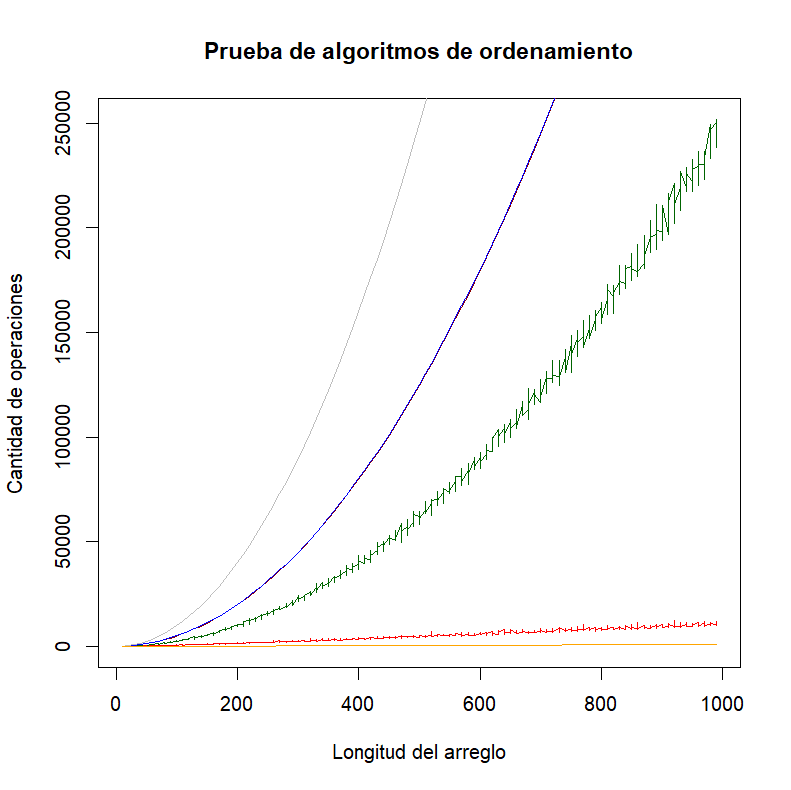
\includegraphics[width=17 cm]{kuchau.png} 
\end{center}

De donde la l\'inea $\textcolor{gray}{gris}$ es el cuadrado de la longitud del arreglo, $\textcolor{blue}{azul}$ ser\'ia el SelectionSort, $\textcolor{deepred}{rojo\> oscuro}$ el BubbleSort, $\textcolor{deepgreen}{verde}$ el InsertionSort, $\textcolor{red}{rojo}$ el QuickSort, y $\textcolor{orange}{naranja}$ la longitud del arreglo.

Podemos concluir varias cosas de la gr\'afica. Los algoritmos de $\textcolor{deepgreen}{\mathrm{Insertion Sort}}$ y $\textcolor{deepred}{\mathrm{BubbleSort}}$ tienen un crecimiento demasiado similar, lo cual tiene sentido, ya que independientemente del orden que tenga un arreglo, siempre realizar\'an una cantidad fija de acuerdo a la longitud del arreglo. Se hace la observaci\'on de que son tan similares, que inclusive la l\'inea de $\textcolor{deepred}{\mathrm{BubbleSort}}$ se aprecia poco, ya que esta empalmada con la de $\textcolor{deepgreen}{\mathrm{Insertion Sort}}$.

  El algoritmo $\textcolor{deepgreen}{\mathrm{Insertion Sort}}$ suele tener un mejor desempe\~no que los algoritmos antes mencionados, ya que si toma ventaja del orden de los n\'umeros y logra realizar menos operaciones. Cabe a recalcar que los tres algoritmos, $\textcolor{blue}{\mathrm{SelectionSort}}$, $\textcolor{deepred}{\mathrm{BubbleSort}}$ y $\textcolor{deepgreen}{\mathrm{Insertion Sort}}$ crecen con una complejidad cuadr\'atica, por ello tienen forma similar a la l\'inea $\textcolor{gray}{gris}$.

Podemos resaltar el gran desempe\~no que tuvo $\textcolor{red}{\mathrm{QuickSort}}$
, ya que en la mayor\'ia de los casos tuvo una cantidad de operaciones considerablemente reducida, en comparaci\'on de los otros tres algoritmos. Comparandolo con la l\'inea $\textcolor{orange}{naranja}$, tenemos que el crecimiento es similar, m\'as no el mismo, ya que se podemos notar que $\textcolor{red}{\mathrm{QuickSort}}$
 crece un poco m\'as r\'apido con el incremento de la longitud de los arreglos.

Como se mencion\'o anteriormente, la complejidad de los algoritmos $\textcolor{blue}{\mathrm{SelectionSort}}$, $\textcolor{deepred}{\mathrm{BubbleSort}}$, $\textcolor{deepgreen}{\mathrm{Insertion Sort}}$ y $\textcolor{red}{\mathrm{QuickSort}}$
 var\'ian de acuerdo a la longitud del arreglo \'o inclusive, por el orden de los elementos del arreglo. Por ello, analizaremos las diagramas de cajas para ver que variaci\'on tienen los algoritmos.


\begin{center}
    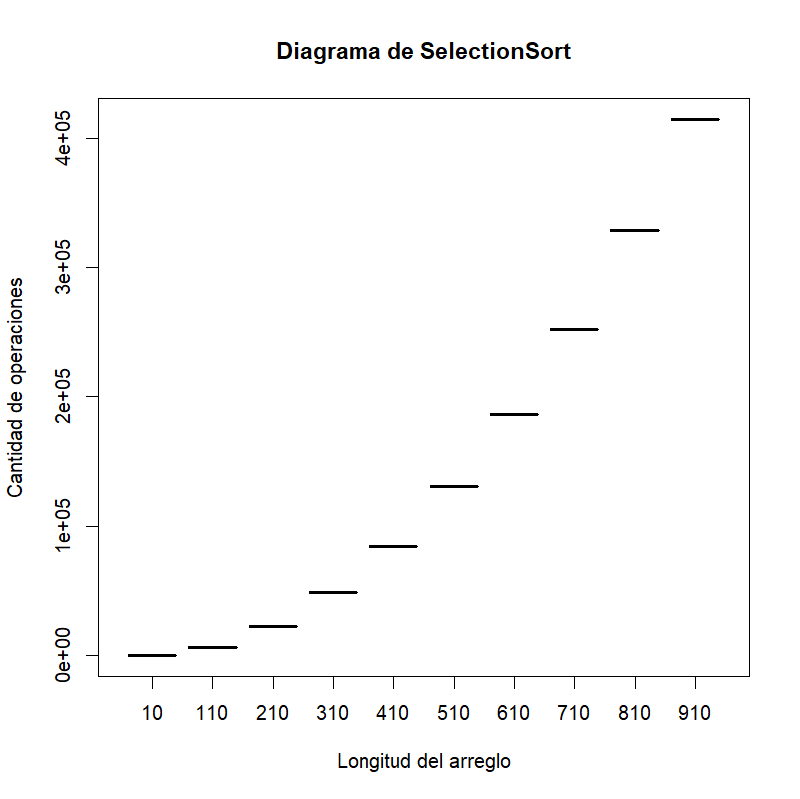
\includegraphics[width=10 cm]{SelectionBox.png} 
\end{center}

\begin{center}
    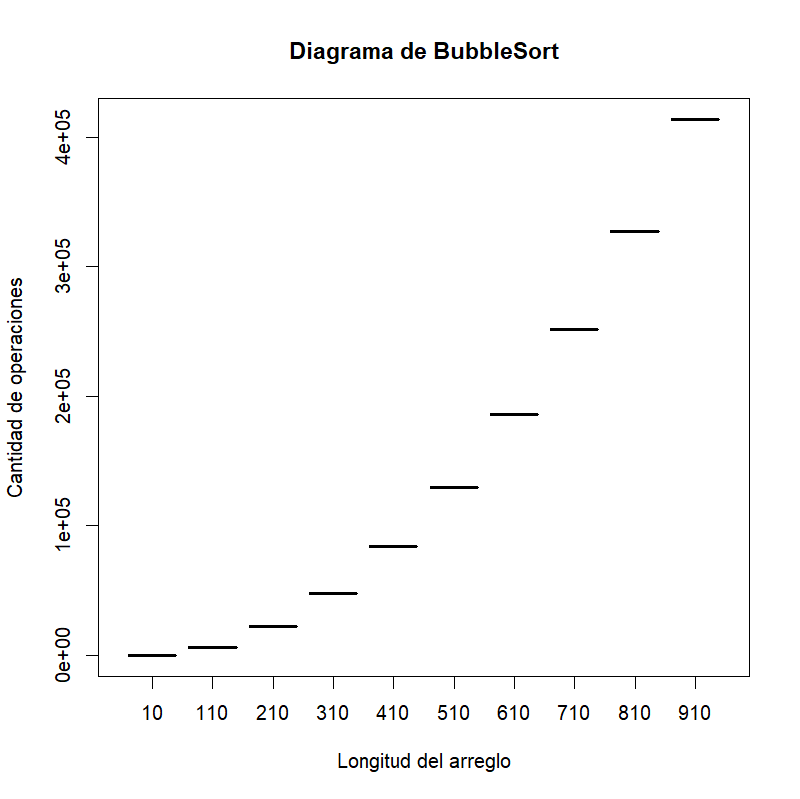
\includegraphics[width=10 cm]{BubbleBox.png} 
\end{center}

\begin{center}
    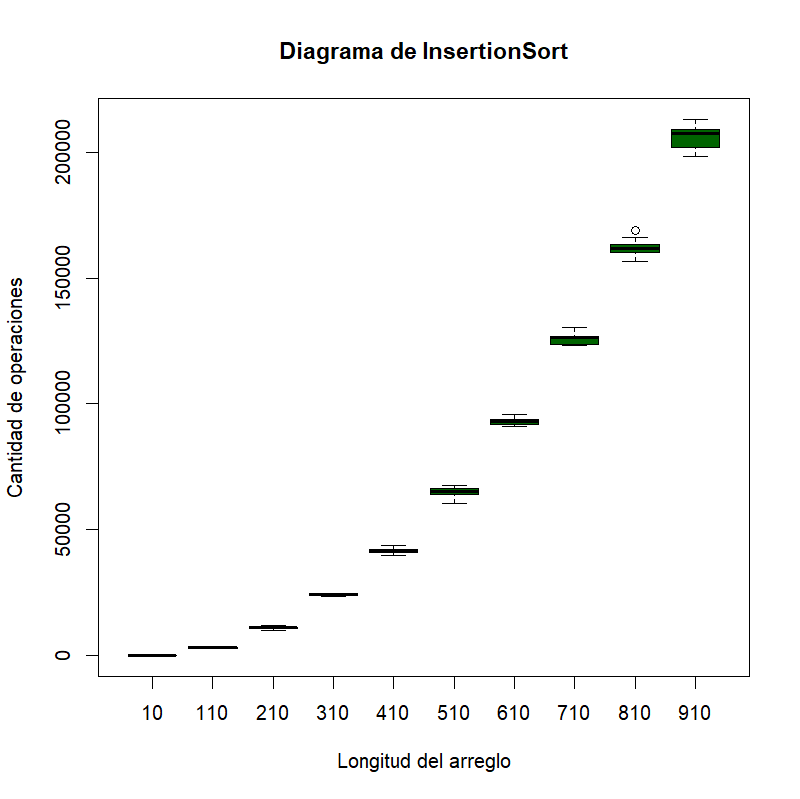
\includegraphics[width=10 cm]{InsertionBox.png} 
\end{center}

\begin{center}
    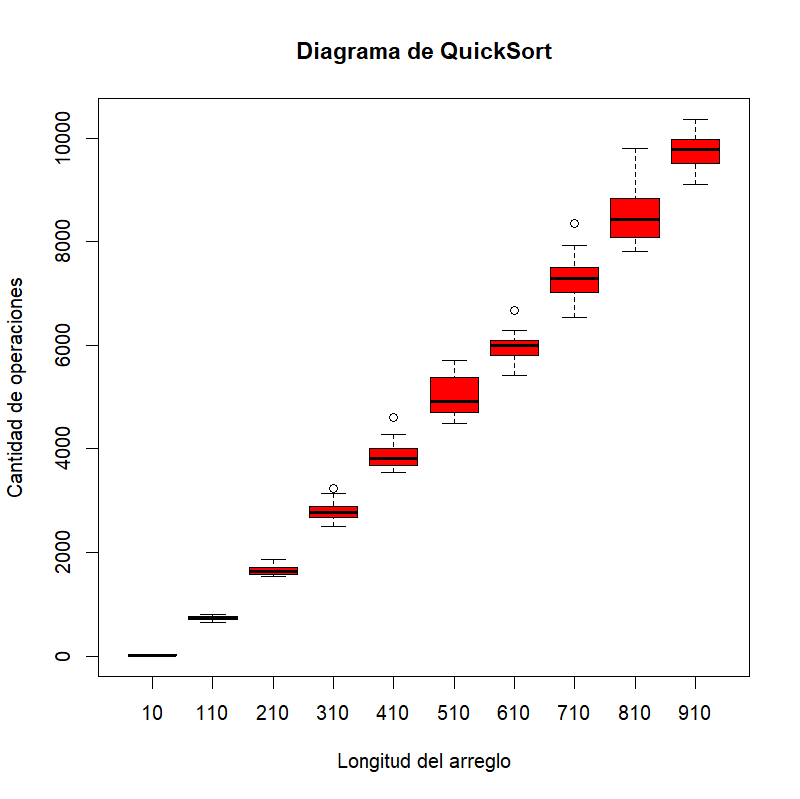
\includegraphics[width=10 cm]{QuickBox.png} 
\end{center}

Las gr\'aficas de $\textcolor{deepgreen}{\mathrm{Insertion Sort}}$ y $\textcolor{deepred}{\mathrm{BubbleSort}}$ son pr\'acticamente iguales, a simple vista no se ve una diferencia. Entre el conjunto de pruebas con la misma longitud, no se logra apreciar ninguna variante de cantidad de operaciones.

De $\textcolor{deepgreen}{\mathrm{Insertion Sort}}$ podemos notar que a medida que la longitud del arreglo aumenta, la variaci\'on aumenta, m\'as no de manera dr\'astica.

En cambio, en la de $\textcolor{red}{\mathrm{QuickSort}}$
 si se notan las variaciones, en donde se logra ver que no siempre se tiene el tiempo \'optimo. 

Vale la pena hacer la observaci\'on de que en el mejor de los casos, en el que el arreglo este ordenado, el algoritmo $\textcolor{deepgreen}{\mathrm{Insertion Sort}}$ corre en tiempo lineal,  mientras que, en el mismo caso, el $\textcolor{red}{\mathrm{QuickSort}}$ se tardar\'ia tiempo cuadr\'atico. 

Por lo tanto, podemos concluir que los algoritmos m\'as eficientes resultaron ser $\textcolor{red}{\mathrm{QuickSort}}$
 e $\textcolor{deepgreen}{\mathrm{Insertion Sort}}$, en donde de acuerdo a la situaci\'on, se utilizar\'ia uno u otro. Por ejemplo, si se desea ordenar un arreglo casi ordenado, es probable que el  $\textcolor{red}{\mathrm{QuickSort}}$
 tardar\'a m\'as que un $\textcolor{deepgreen}{\mathrm{Insertion Sort}}$. Aunque, de manera general, se espera que el $\textcolor{red}{\mathrm{QuickSort}}$
 tenga complejidad  $\mathcal{O}(nlog{}n)$ y el $\textcolor{deepgreen}{\mathrm{Insertion Sort}}$ $\mathcal{O}(n^2)$.


Antes de verlo en pr\'actica no me sorprender\'ia que la computadora ordenar\'a miles de datos en cuesti\'on de segundos, pero al simular el ordenamiento de los 1500 arreglos, resulto que se tard\'o varios minutos en ordenarlos con los cuatro algoritmos. Me result\'o interesante, ya que despu\'es de eso, ordene solo con $\textcolor{red}{\mathrm{QuickSort}}$ y la diferencia fue abrumadora, ya que en tan solo segundos se hab\'ian ordenado.

En estas pruebas fueron miles, pero tenemos que tener en cuenta que en la vida real puede que se necesite ordenar arreglos demasiados extensos,  y por ello es conveniente aprender y desarrollar mejores formas de realizar las cosas, en este caso, ordenar.


\section{Detalles de implementaci\'on}

Al principio no sab\'ia bien que onda con la sintaxis de Python, qu\'e tipo de cosas pod\'ia hacer en Python, c\'omo pod\'ia hacer aquello tipo de cosas, qu\'e similitudes tiene con C++, c\'omo leer datos y c\'omo imprimir, estas y muchas otras m\'as dudas me invadieron al principio. Pero viendo la aplicaci\'on de las funciones y operaciones, los ejemplos del profe y de internet, pues fu\'i aprendiendo y ya pod\'ia adaptarlo de acuerdo a lo que necesitar\'a en el momento. 

Para implementar el $\textcolor{blue}{\mathrm{SelectionSort}}$ y el $\textcolor{deepred}{\mathrm{BubbleSort}}$ no v\'i necesario indagar sobre funciones raras, o detalles sobre alguna funci\'on, con el uso del $\pythoninline{for}$, $\pythoninline{range}$, variables auxiliares y unas cuantas asignaciones logre implementar los algoritmos.

Para implementar $\textcolor{deepgreen}{\mathrm{Insertion Sort}}$ tuve el problema de disminuir el indice uno por uno.
Aun teniendo la opci\'on de simular el $\pythoninline{for}$ con un $\pythoninline{while}$ para poder disminuir de uno en uno, prefer\'i investigar si hab\'ia alguna forma para lograrlo, en donde encontre que al hacer $\pythoninline{range(a,b,-1)}$, en donde en vez de tener los n\'umeros en el orden de $\{a,\> a+1,\>\dots,\>b-1\}$ (Con $a<b$), se tiene $\{a,\>a-1,\>\dots,b+1\}$(Con $a>b$) que era lo que buscaba en el momento.

Para implementar $\textcolor{red}{\mathrm{QuickSort}}$, con entender la recursividad que se realizaba y demostrar que el caso base de tener el elemento vac\'io (o de un s\'olo elemento) era suficiente, ayud\'o a que no se me dificultar\'a la implementaci\'on del mismo. Aqu\'i hice uso de la concatenaci\'on de arreglos, lo cual me hace gracia lo sencillo que es en Python, mientras que en C++ se necesita m\'as l\'ineas. 
\end{document}